\section{Output}

\subsection{HDF5 Output}

By default, M3D-C1 will output data to a HDF5 file named \texttt{C1.h5}.  The file is organized as follows:

\begin{itemize}
\item state variables
\item \texttt{scalars/}
\item \texttt{equilibrium/}
\item \texttt{time\_\#\#\#/}
\end{itemize}  

\subsubsection{State variables}

\subsubsection{The \texttt{scalars/} group}

The \texttt{scalars/} group contains one-dimensional time series data,
output at every MHD timestep.  Some of the time series that are output
include the following:

\begin{tabular}{lll}
\textbf{Scalar}   & \textbf{Units} & \textbf{Description} \\
\hline
time              & $t_0$          & The physical time at each MHD timestep\\
dt                & $t_0$          & The physical time per MHD timestep\\ 
loop\_voltage     & $V_0$          & The loop voltage applied at the domain boundary\\
toroidal\_current & $I_0$          & The total toroidal current in the MHD region\\
particle\_number  & $n_0 L_0^3$    & The total number of main ions in the MHD region\\
electron\_number  & $n_0 L_0^3$    & The total number of electrons in the MHD region\\
power\_injected   & $p_0 L_0^3 / t_0$ & The total power from the heat source in the MHD region
\end{tabular}

For simulations that make use of the KPRAD module, the following time
series are also output:

\begin{tabular}{lll}
\textbf{Scalar}   & \textbf{Units} & \textbf{Description} \\
\hline
radiation & $p_0 L_0^3 / t_0$ & Total power loss due to all radiation sources\\
line\_rad & $p_0 L_0^3 / t_0$ & Power loss due to line radiation\\
brem\_rad & $p_0 L_0^3 / t_0$ & Power loss due to bremsstrahlung\\
ion\_loss & $p_0 L_0^3 / t_0$ & Power loss due to ionization\\
reck\_rad & $p_0 L_0^3 / t_0$ & \\
recp\_rad & $p_0 L_0^3 / t_0$ & \\
kprad\_n  & $n_0 L_0^3$ & Total number of impurity nuclei (both ionized and neutral)\\
kprad\_n0 & $n_0 L_0^3$ & Total number of neutral impurity atoms\\
kprad\_dt & $t_0$       & Time step of KPRAD subcycle
\end{tabular}


\subsubsection{The \texttt{equilibrium/} and \texttt{time\_\#\#\#/} groups}

The \texttt{equilibrium/} and \texttt{time\_\#\#\#/} groups contain the
mesh and field data upon initialization (\texttt{equilibrium/} and
\texttt{time\_000/}) and at each field output time slice
(\texttt{time\_\#\#\#}).  The number of MHD timesteps per field output
time slice is determined by the C1input parameter \texttt{ntimepr}.

In calculations with eqsubtract=1, the \texttt{equilibrium/} group
contains the equilibrium part of the fields whereas \texttt{time\_\#\#\#/}
contain the perturbed part of the fields.

The data in \texttt{equilibrium/} and \texttt{time\_\#\#\#} are written to
separate files named \texttt{equilibrium.h5} and
\texttt{time\_\#\#\#.h5}.  These files are linked to \texttt{C1.h5} using
the linking feature of HDF5 so that the data can be accessed as if it
were a regular group in \texttt{C1.h5}.

\begin{tabular}{lll}
\textbf{Variable} & \textbf{Units} & \textbf{Description}\\
\hline
time              & $t_0$ & Physical time of time slice\\
nspace            & 1     & 2 for 2D / complex; 3 for 3D simulations\\
ntimestep         & 1     & MHD timestep associated with this times lice\\
version           & 1     & Version number for output data\\
mesh/             &       & Mesh data group\\
mesh/nelms        & 1     & Number of mesh elements\\
mesh/period       & 1     & Toroidal period of mesh\\
mesh/ifull\_torus & 1     & 1 if full-torus simulation; 0 if partial-torus simulation\\
mesh/nperiods     & 1     & If partial torus, number of periods per full torus\\
mesh/phi          & 1     & 1D array containing the toroidal angles of the toroidal planes\\
mesh/elements     &       & 2D array containing mesh data\\
mesh/adjacency    &       & 2D array containing adjacency data\\
fields/           &       & Group containing field data
\end{tabular}

\begin{figure}
\begin{center}
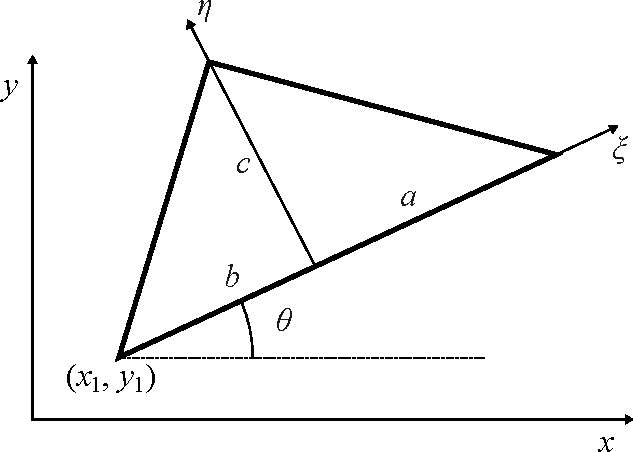
\includegraphics{figures/C1_element.pdf}
\caption{\label{fig:C1}The geometry of a mesh element in the toroidal plane\cite{Jardin04}}
\end{center}
\end{figure}

\paragraph{\texttt{mesh/elements}} is a 2D array consisting of
\texttt{nelms} rows (one per mesh element), with 8 (for 2D
simulations) or 10 (for 3D simulations) columns:

\[ a, b, c, \theta, x_1, y_1, \text{ibound}, \text{izone}, d, \varphi_1 \]

The first five columns ($a$ through $y_1$) describe the geometry of
the element in the toroidal plane, as illustrated in
figure~\ref{fig:C1}.  $d$ and $\varphi_1$ represent the toroidal
extent of the element and the toroidal coordinate of the first
bounding plane (in radians if itor=1, in units of $L_0$ otherwise),
and are only present for 3D simulations.

\paragraph{Fields/} is a group containing the field data.  Each field
is a 2D array consisting of \texttt{nelms} rows (one per element) and
20 (in 2D) or 80 (in 3D) columns, representing the coefficients of
each shape function within the given mesh element.

The field $\phi$ at the coordinate system $(\xi,\eta,\zeta)$ local to the mesh element is given by
\[ 
  \phi(\xi,\eta,\zeta) = \sum_{j=0}^{J} \sum_{i=1}^{20} a_{i + 4(j-1)} \xi^{m_i} \eta^{n_i} \zeta^j
\]
where
\begin{eqnarray*}
   m & = & \{0,1,0,2,1,0,3,2,1,0,4,3,2,1,0,5,3,2,1,0 \}\\
   n & = & \{0,0,1,0,1,2,0,1,2,3,0,1,2,3,4,0,2,3,4,5 \}\\
\end{eqnarray*}
and where $J=3$ for 3D simulations and $J=0$ for 2D / complex simulations.

The fields that are written include the following.  (Note that in 2D
complex simulations, these field names contain the real part of the
field data; for each field an additional field with the suffix "\_i"
is written to contain the imaginary part.)

\begin{tabular}{llll}
\textbf{Field} & \textbf{Units (itor=1)} & \textbf{Units (itor=0)} & \textbf{Description}\\
\hline
psi  & $B_0 L_0^2$ & $B_0 L_0$   & $\psi$\\
I    & $B_0 L_0$   & $B_0$       & $F$ \\
f    & $B_0 L_0$   & $B_0 L_0^2$ & $f$ \\
phi  & $v_0$       & $v_0 L_0$   & $U$ \\
V    & $v_0/L_0$   & $v_0$       & $\omega$ \\
chi  & $v_0 L_0^3$ & $v_0 L_0$   & $\chi$ \\
P    & $p_0$       & $p_0$       & $p$ \\
Pe   & $p_0$       & $p_0$       & $p_e$ \\
ti   & $T_0$       & $T_0$       & $T_i$ \\
te   & $T_0$       & $T_0$       & $T_e$ \\
den  & $n_0$       & $n_0$       & $n_i$ \\
ne   & $n_0$       & $n_0$       & $n_e$
\end{tabular}

